\documentclass{beamer}

% Theme
\usetheme{Madrid}
\usecolortheme{default}
\setbeamertemplate{navigation symbols}{}
\setbeamertemplate{bibliography entry title}{}
% Packages
\usepackage{amsmath, amssymb}
\usepackage{graphicx}
\nocite{*}
\bibliographystyle{plain}  % or another style like alpha, ieeetr, etc.
% Title Page
\title[Implicit Loss Fine-Tuning]{Fine-tuning with implicit loss}
\author{Łukasz Adamowicz}
\institute[]{M2 Mathématiques, Modélisation et Apprentissage\\ Université Paris Cité \\ Internship at Hamprecht Lab, IWR Heidelberg \\
}
\date{\today}
\begin{document}

% Title slide
\begin{frame}
  \titlepage
\end{frame}

% Outline
\begin{frame}{Outline}
  \tableofcontents
\end{frame}


%------------------------------------------------------
\section{Problem Statement}
\begin{frame}{General Optimization Problem}
  \begin{itemize}
    \item Our model: $E(\theta, M, p)$.
    \item $p_{\theta,i}$ are fixed points:
    \[
      p_{\theta,i} = \arg\min_{p:\langle w_i,p \rangle = N_i} E(\theta, M_i, p).
    \]
    \item Loss: $L(\theta) = \sum_{i=1}^{n} L_i(p_{\theta,i}) = \sum_{i=1}^{n} \frac{1}{2} \|p_{\theta,i} - p_{gs,i}\|^2$.
    \item Keywords: bilevel optimization, stochastic bilevel optimization, Deep Equilibrium Models
  \end{itemize}
\end{frame}

\begin{frame}{Single Molecule Optimization Problem}
  \begin{itemize}
    \item For a single molecule $M$:
    \item Fixed point : $$p_{\theta} = \arg\min_{p:\langle w,p \rangle = N} E(\theta, p)$$.
    \item Loss: $L(\theta) = L(p_{\theta}) = \frac{1}{2}\|p_{\theta} - p_{gs}\|^2$.
    \item Goal: Minimize loss function $L(\theta)$.
    \item In bilevel optimization terms minimizing $L(p_\theta)$ is called an outer problem and minimizing $E(\theta, p)$ is an inner problem.
  \end{itemize}
\end{frame}

%------------------------------------------------------
\section{Jacobian Approach}
\begin{frame}{Jacobian Approach}
  \begin{itemize}
    \item Formula for gradient of the loss is:
    \[
      \frac{\partial L(p_{\theta})}{\partial \theta} = -(p_{\theta}-p_{gs}) \cdot \left(\frac{\partial}{\partial p}\mathcal{P}\big(\nabla_p E(\theta, p)\big)\right)^{-1} \cdot \frac{\partial}{\partial \theta}\big(\mathcal{P}\nabla_p E(\theta, p)\big)
    \]
    \item  $\mathcal{P}$ is the projection operator onto subspace $\langle w,p \rangle = 0$.
    \item Hessian $ \left(\frac{\partial}{\partial p}\mathcal{P}\big(\nabla_p E(\theta, p)\big)\right)$ is \textbf{not} invertible, we utilize pseudoinverse instead.
    \item In practice, we solve the linear equation $ y \cdot \left(\frac{\partial}{\partial p}\mathcal{P}\nabla_p E(\theta, p)\right) = -(p_{\theta}-p_{gs})$.
    \item This is done with matrix-free methods, because materializing the matrix is slow.
  \end{itemize}
\end{frame}

\begin{frame}{Jacobian Results}
  \begin{itemize}
    \item Training is very unstable, depends on inner problem hyperparameters.
    \item Conjugate gradient method failed to solve linear equation
    \item Even when training loss decreased, it did not improve network metrics.
    \item Hessian has big both big ($\approx 1000$) and small ($\approx 0.001$) eigenvalues, plain gradient descent on $\|y \cdot \left(\frac{\partial}{\partial p}\mathcal{P}\nabla_p E(\theta, p)\right) + (p_{\theta}-p_{gs})\|^2$ fails, resorted to ADAM.
    \item Overall, Jacobian approach did not work.
  \end{itemize}
\end{frame}



%------------------------------------------------------
\section{Equilibrium Propagation}
\begin{frame}{Equilibrium Propagation}
  \begin{itemize}
    \item Alternative gradient estimation method (see bibliography for details).
    \item Define total energy: $T(\theta, p, \beta) = E(\theta, p) + \beta \frac{1}{2}\|p-p_{gs}\|^2 = E(\theta, p) + \beta L(p)$
    \item Define $p_{\theta}^{\beta}$ as the fixed point of $T$.
    \[
      p_{\theta}^{\beta} = \arg\min_{p:\langle w,p \rangle = N} T(\theta, p, \beta)
    \]
    \item Gradient formula:
    \[
      \frac{d}{d\theta} L(p_{\theta}) = \lim_{\beta \to 0} \frac{1}{\beta} \Big[ \partial_{\theta}T(\theta, p^{\beta}_{\theta}, \beta) - \partial_{\theta}T(\theta, p^{0}_{\theta}, 0) \Big].
    \]
    \item Approximate gradient as finite difference of right-hand side (numerical derivative)
  \end{itemize}
\end{frame}

\begin{frame}{Equilibrium Propagation Results}
  \begin{itemize}
    \item Fine-tuned single molecule succesfully.
    \item Can work, when Jacobian approach fails
    \item Slower than Jacobian approach.
    \item Original contribution: implement in DFT setting, comparison with Jacobian (IFT) approach
    \item More details and derivation in the report.
  \end{itemize}

\end{frame}

\begin{frame}

 \begin{center}
    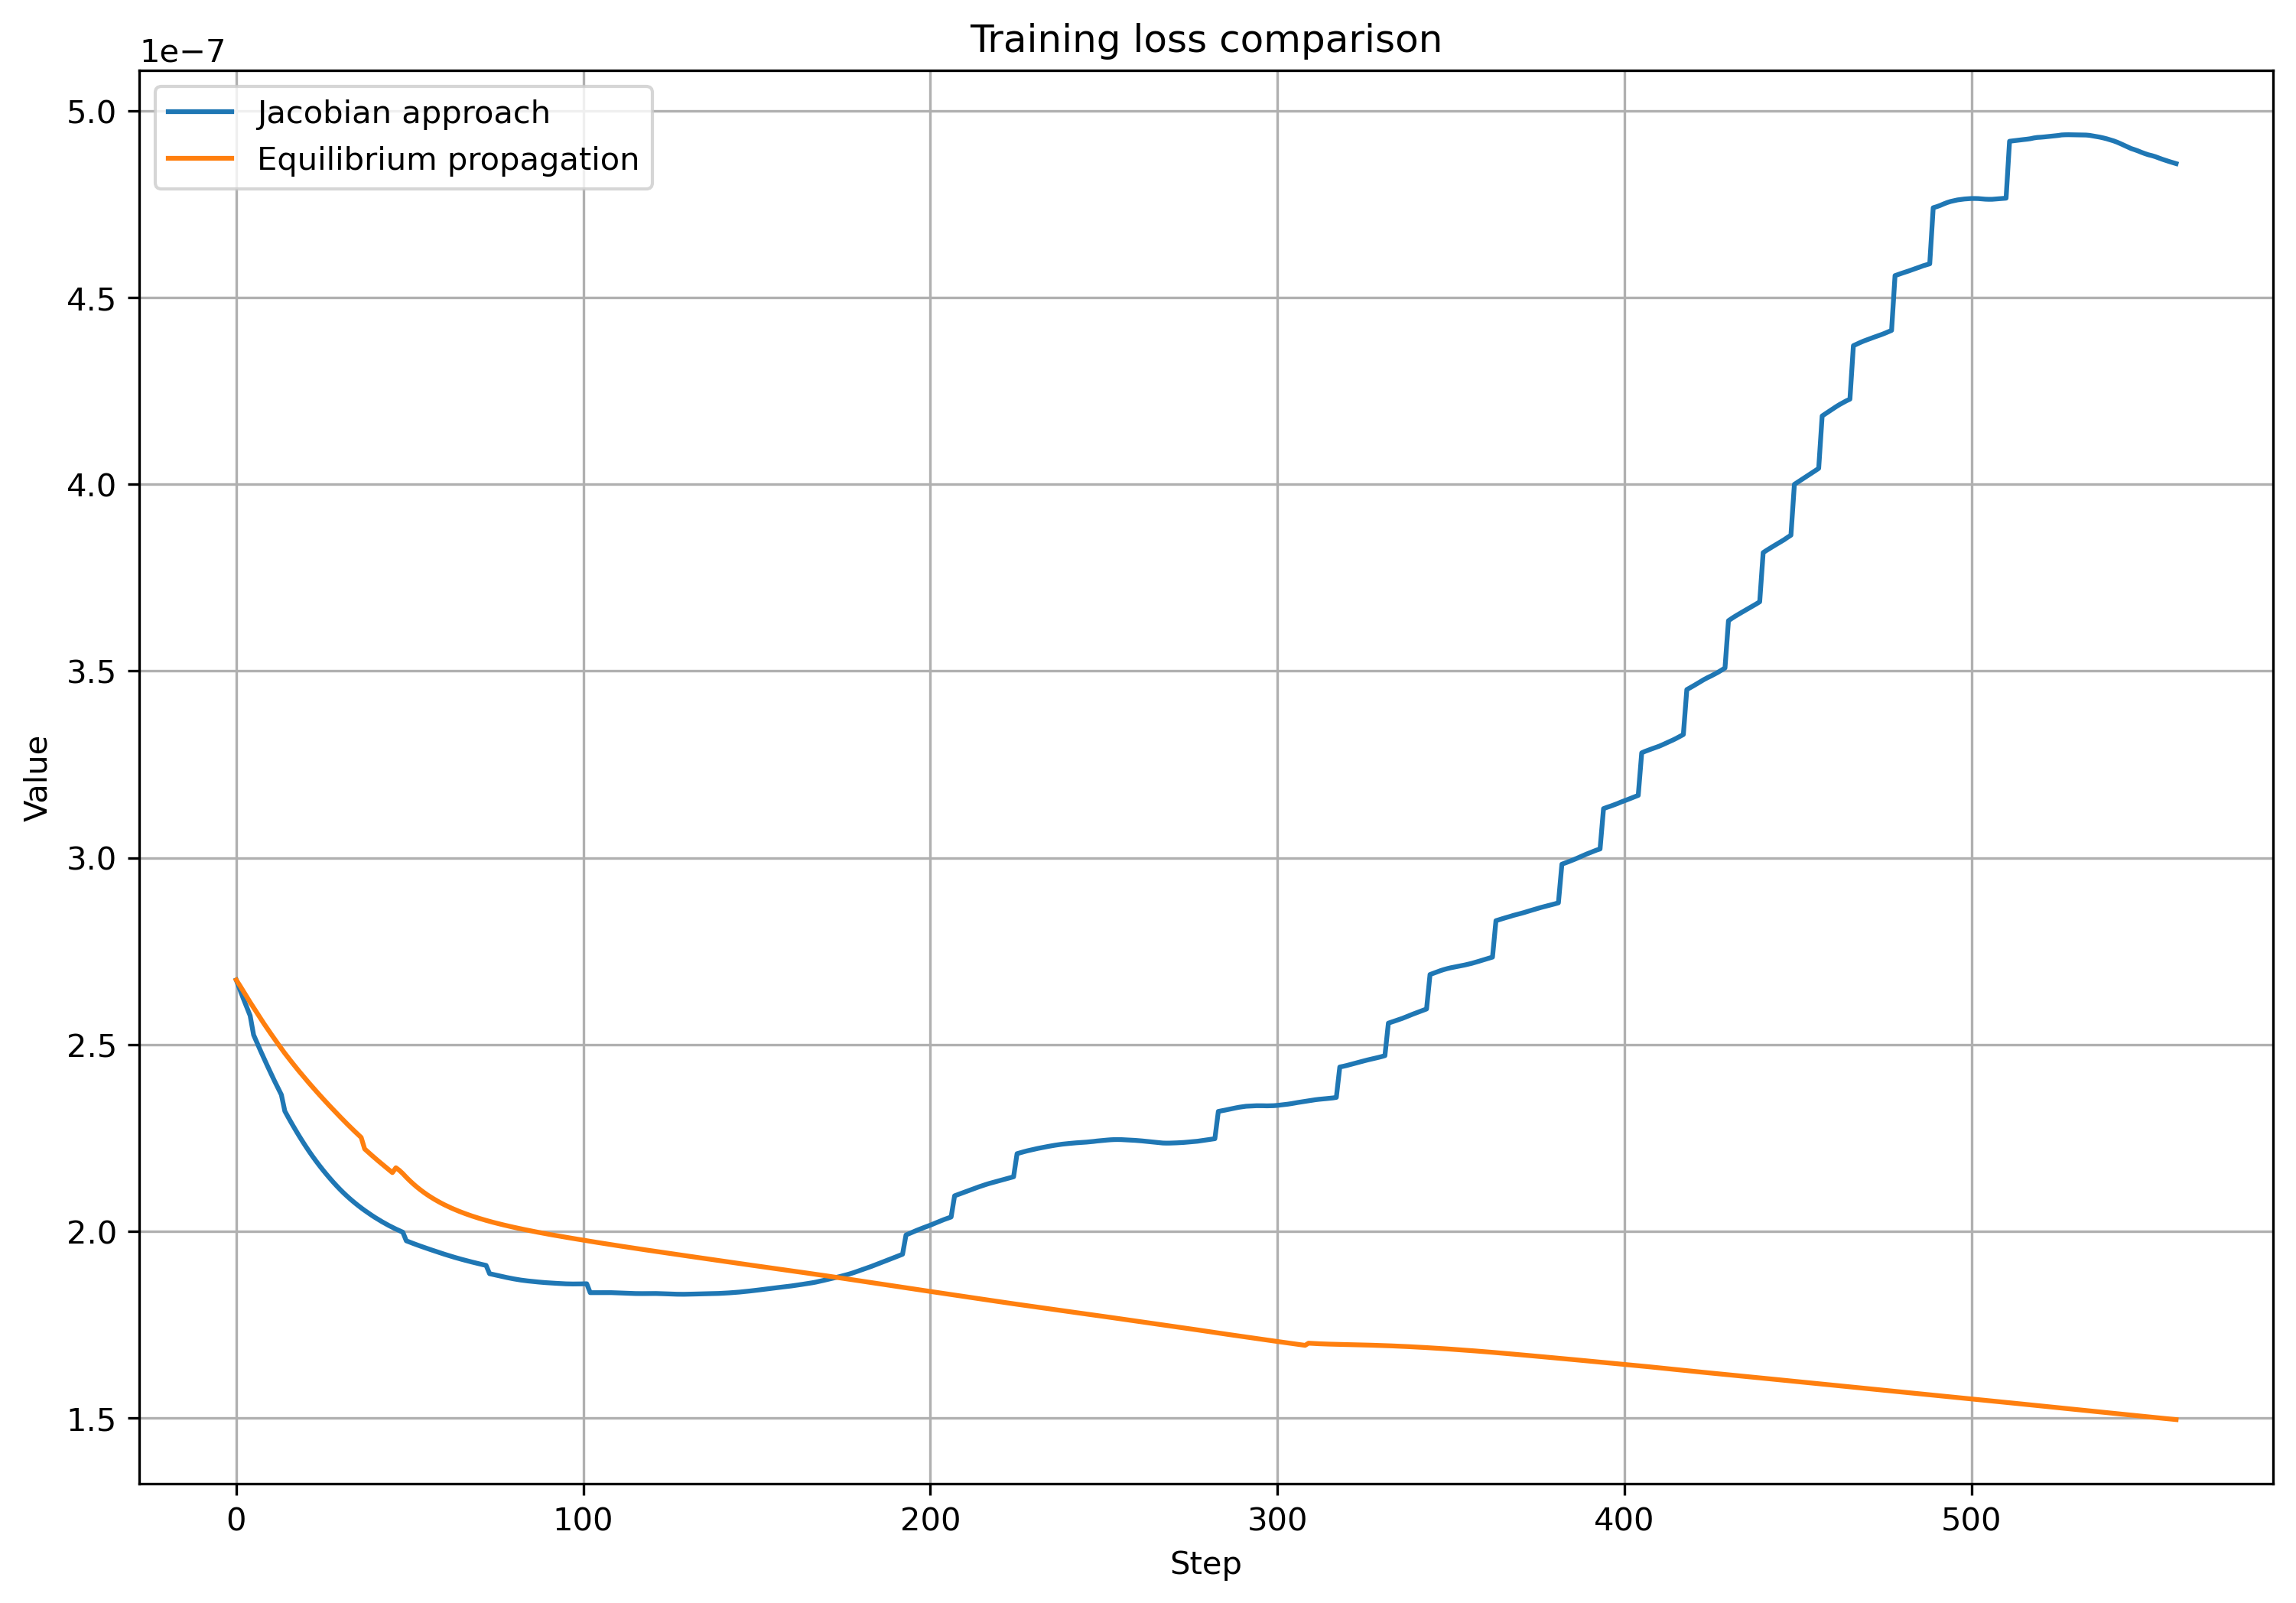
\includegraphics[width=0.8\textwidth]{images/loss_comparison.png} % Jacobian vs EqProp training loss
  \end{center}
\end{frame}

%------------------------------------------------------
\section{Stability Issues and Fixed Point Correction}
\begin{frame}{Stability Issues}
  \begin{itemize}
    \item Training stability deteriorates over time (known issue in DEQ models).
    \item Fixed point search takes longer and longer during training.
    \item There are techniques for alleviating the issue
    \item Appears both in Jacobian and EqProp approaches.
    \item Appears only, when trying to fine-tune on multiple molecules.
  \end{itemize}
\end{frame}

\begin{frame}{Fixed Point Correction}
  \begin{itemize}
    \item Technique: include intermediate trajectory points in loss. Taken from DEQ literature.
    \item Inner problem trajectory is $p_1, \ldots, p_T \approx p_\theta$.
    \item Uniformly choose $n$ intermediate points and modify the loss function as
    \[
      L_{FPC}(\theta) = \sum_{k=1}^{n} \gamma^{n-k} L(p_{i_k}),
    \]
    \item Treat $p_{i_k}$ as fixed points and calculate gradient using Jacobian approach.
    \item Helps stabilize training, but may reduce performance.
    \item Original contribution: Adapt to EqProp, add stochasticity.
  \end{itemize}

\end{frame}

\begin{frame}
   \begin{center}
    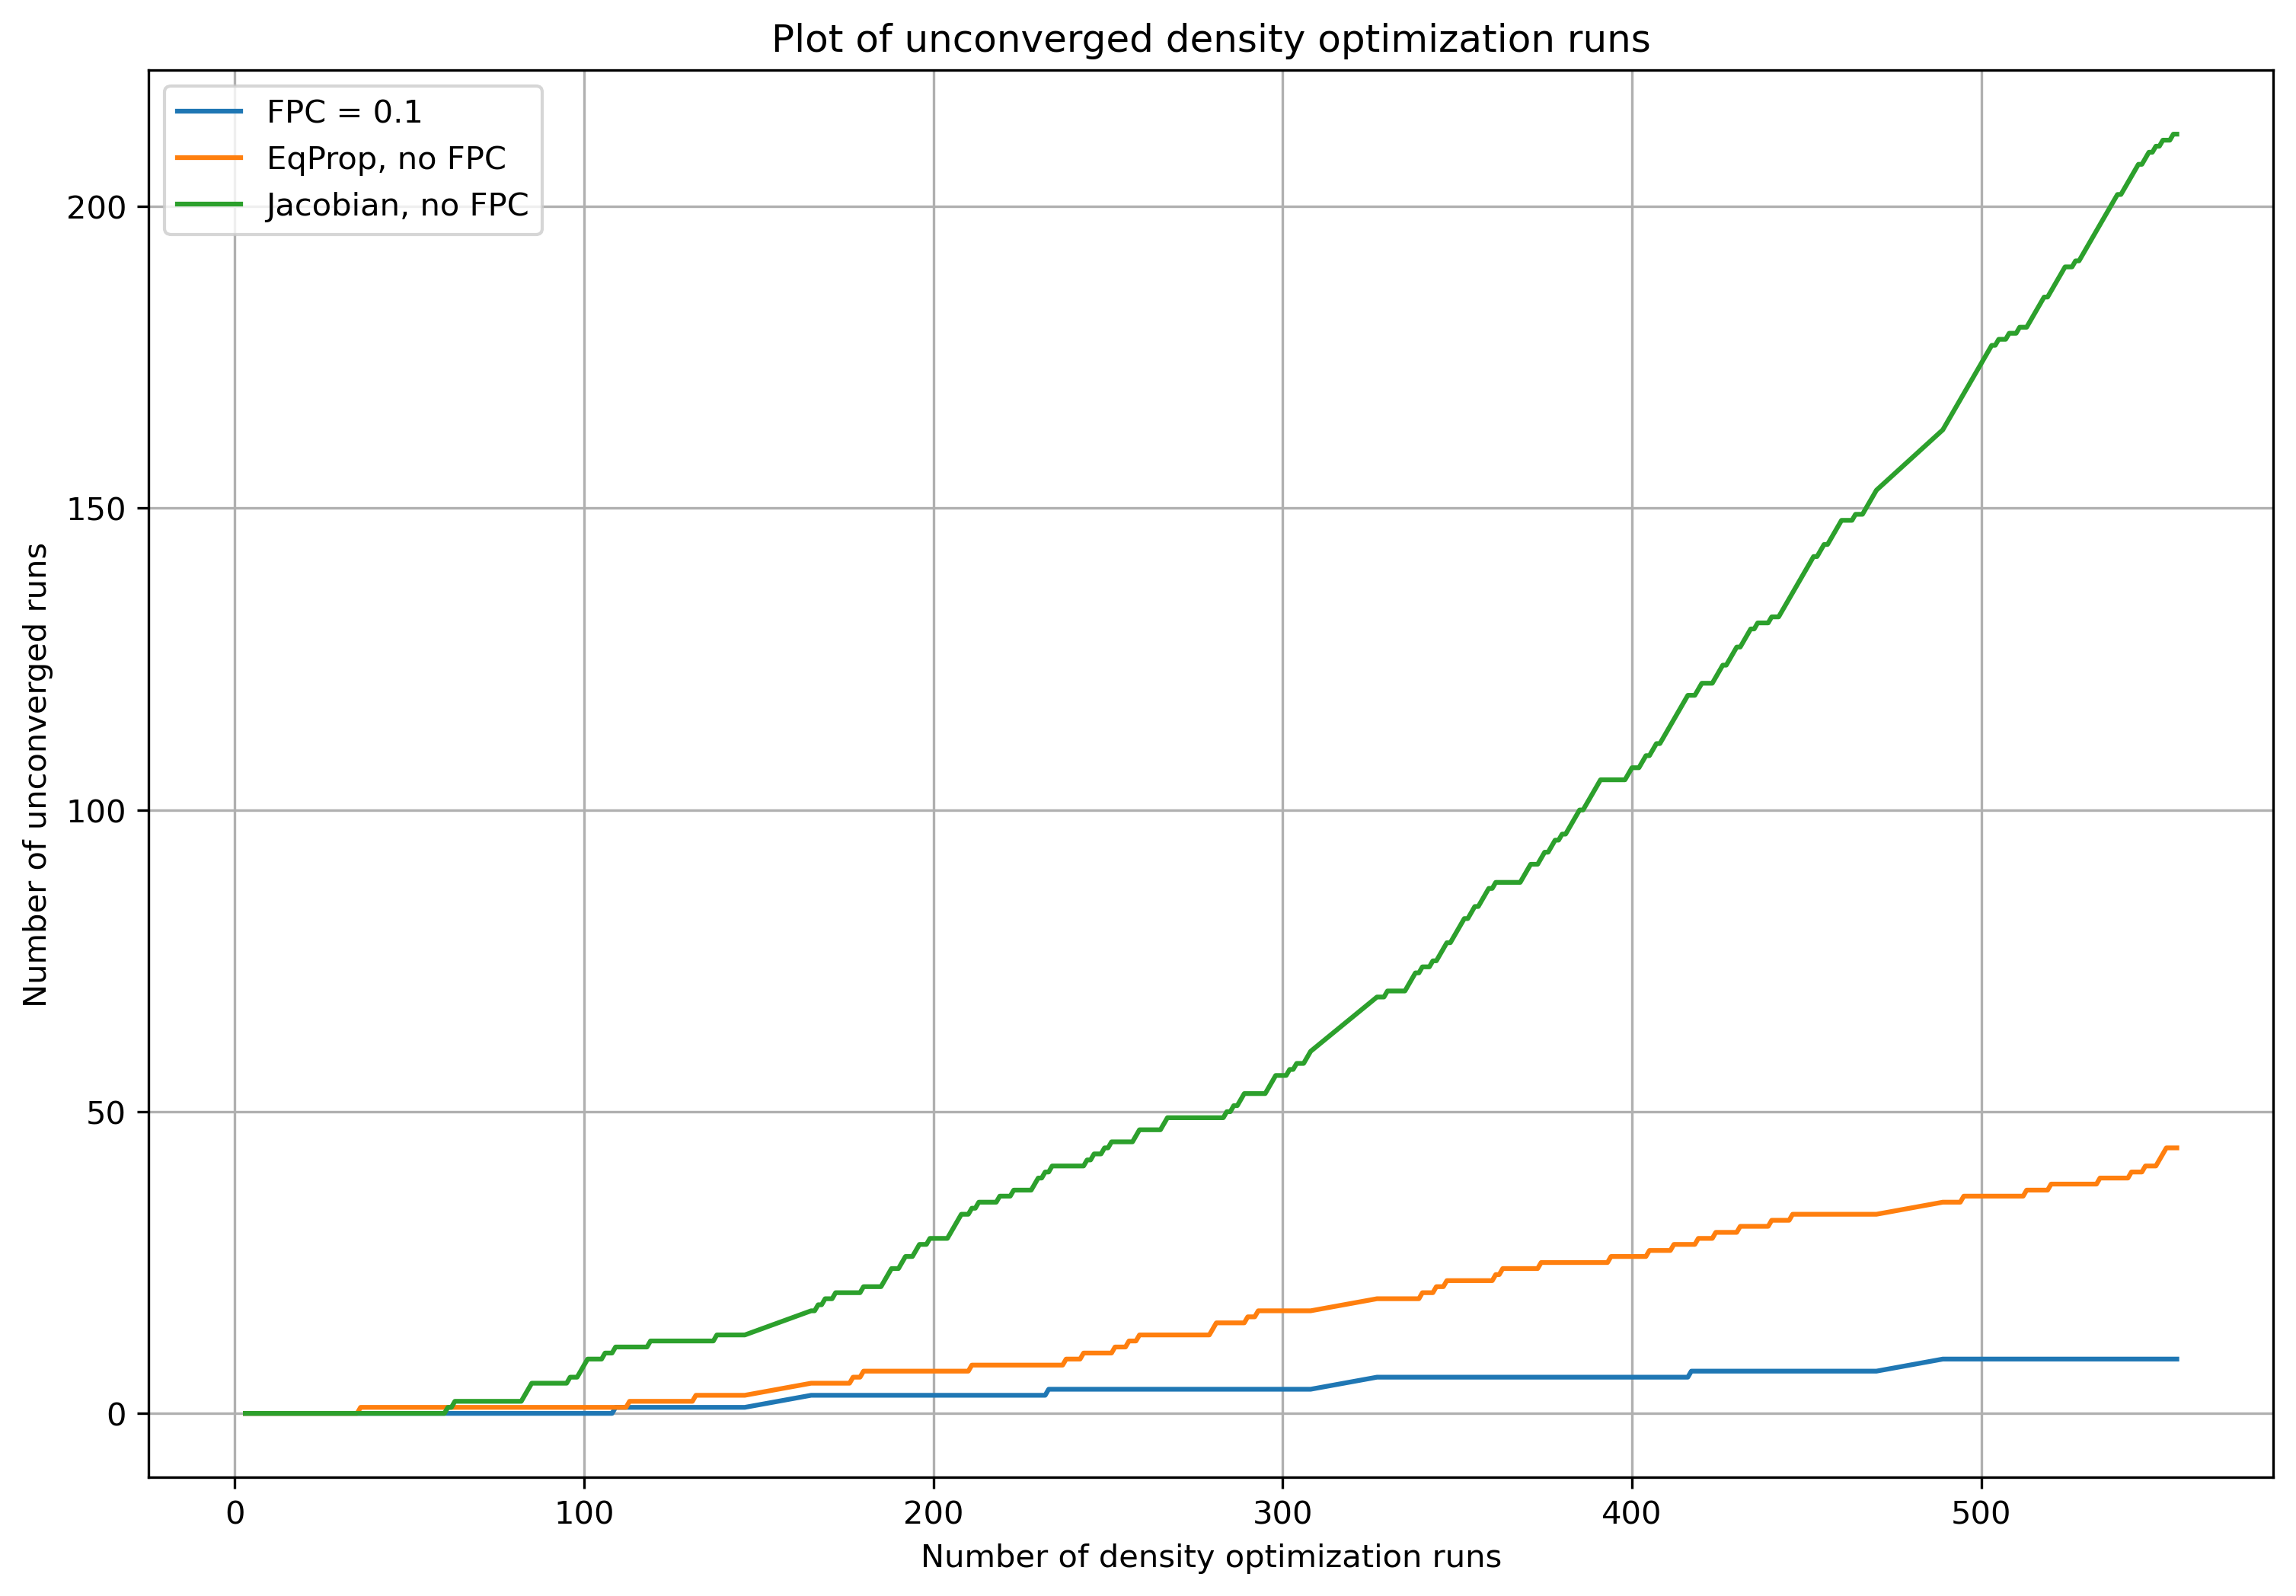
\includegraphics[width=0.8\textwidth]{images/stability_plot.png} % Stability plot
  \end{center}
\end{frame}

%------------------------------------------------------
\section{Conclusions}
\begin{frame}{Conclusions}
  \begin{itemize}
    \item Jacobian approach: not working right now, badly conditioned problem.
    \item Equilibrium propagation: works on single molecules.
    \item Biggest problem is training stability, additional treatment is needed.
    \item Training is very slow

  \end{itemize}
\end{frame}

\begin{frame}{End}
\begin{center}
 Thank You for coming
\end{center}
\end{frame}
\begin{frame}[allowframebreaks]{References}
\nocite{*}
\bibliographystyle{plain}
\bibliography{./references.bib}
\end{frame}

%------------------------------------------------------
\appendix
\section{Appendix}
\begin{frame}{Jacobian Gradient Derivation - Part 1}
  \begin{itemize}
    \item Starting from loss function: $L(\theta) = \frac{1}{2}\|p_{\theta} - p_{gs}\|^2$.
    \item Using chain rule: $\frac{\partial L}{\partial \theta} = \frac{\partial L}{\partial p_{\theta}} \cdot \frac{\partial p_{\theta}}{\partial \theta}$.
    \item First term is straightforward: $\frac{\partial L}{\partial p_{\theta}} = (p_{\theta} - p_{gs})$.
    \item For second term, we need the implicit function theorem.
  \end{itemize}
\end{frame}

\begin{frame}{Jacobian Gradient Derivation - Part 2}
  \begin{itemize}
    \item At fixed point, we have: $\mathcal{P}\nabla_p E(\theta, p_{\theta}) = 0$.
    \item Differentiating this constraint with respect to $\theta$:
    \begin{align}
      \frac{\partial}{\partial \theta}\left[\mathcal{P}_{\langle w,p \rangle = N}\nabla_p E(\theta, p_{\theta})\right] &= 0 \\
      \frac{\partial}{\partial p}\mathcal{P}_{\langle w,p \rangle = N}\nabla_p E(\theta, p_{\theta}) \cdot \frac{\partial p_{\theta}}{\partial \theta} + \frac{\partial}{\partial \theta}\mathcal{P}_{\langle w,p \rangle = N}\nabla_p E(\theta, p_{\theta}) &= 0
    \end{align}
    \item Solving for $\frac{\partial p_{\theta}}{\partial \theta}$:
    \begin{align}
      \frac{\partial p_{\theta}}{\partial \theta} &= -\left(\frac{\partial}{\partial p}\mathcal{P}_{\langle w,p \rangle = N}\nabla_p E(\theta, p_{\theta})\right)^{-1} \cdot \frac{\partial}{\partial \theta}\mathcal{P}_{\langle w,p \rangle = N}\nabla_p E(\theta, p_{\theta})
    \end{align}
  \end{itemize}
\end{frame}

\begin{frame}{Jacobian Gradient Derivation - Part 3}
  \begin{itemize}
    \item Substituting back into our chain rule formula:
    \begin{align}
      \frac{\partial L}{\partial \theta} &= (p_{\theta} - p_{gs}) \cdot \frac{\partial p_{\theta}}{\partial \theta} \\
      &= -(p_{\theta} - p_{gs}) \cdot \left(\frac{\partial}{\partial p}\mathcal{P}\nabla_p E(\theta, p_{\theta})\right)^{-1} \cdot \frac{\partial}{\partial \theta}\mathcal{P}\nabla_p E(\theta, p_{\theta})
    \end{align}

  \end{itemize}
\end{frame}

\begin{frame}{Equilibrium Propagation Derivation - Part 1}
  \begin{itemize}
    \item Define perturbed energy function: $T(\theta,p,\beta)=E(\theta,p)+\beta L(p)$.
    \item Define $p_{\theta}^{\beta}$ as the fixed point of this perturbed energy:
    \[
      p_{\theta}^{\beta} = \arg\min_{p:\langle w,p \rangle = N} T(\theta, p, \beta)
    \]
    \item Note that $p_{\theta}^{0} = p_{\theta}$ (the original fixed point).
    \item Our goal: compute $\frac{d}{d\theta}L(p_{\theta})$.
  \end{itemize}
\end{frame}

\begin{frame}{Equilibrium Propagation Derivation - Part 2}
  \begin{itemize}
    \item Define function $G(\theta,\beta) = T(\theta,p_{\theta}^{\beta}, \beta)$.
    \item There's symmetry of second derivatives $\frac{d}{d\beta}\frac{d}{d\theta} $ at $\beta = 0, \theta = \theta$

  \end{itemize}
\end{frame}

\begin{frame}{Equilibrium Propagation Derivation - Part 3}
  \begin{itemize}
    \item $\frac{dG}{d\beta×} = \frac{\partial T}{\partial \beta} + \frac{\partial T}{\partial p} \frac{d p_\theta^\beta}{d\beta×},$ but the second term vanishes at $p = p_\theta^\beta$.
    \item $ \frac{\partial T}{\partial \beta}\big|_{\beta = 0} = L(p_\theta)$
  \end{itemize}
\end{frame}



\end{document}
